\chapter{Granular flows}

\ifpdf
    \graphicspath{{Chapter2/figs/raster/}{Chapter2/figs/pdf/}{Chapter2/figs/}}
\else
    \graphicspath{{Chapter2/figs/vector/}{Chapter2/figs/}}
\fi

\section{Introduction}

A granular material is a conglomeration of a large number of discrete solid 
grains of sizes greater than $1\mu m$ whose behaviour is governed by 
frictional contacts and inelastic collisions. A schematic representation of the 
size range of the granular materials is presented in~\cref{fig:granular}. 
Granular materials, characterized by interaction between individual grains, 
lie between two extremes scales: the molecular-scale range predominated by 
electrostatic force, i.e. Van der Waals forces, and the continuum scale which 
is described by the bulk property of the material. In various soil 
classification systems adopted in soil mechanics, sand is classified as a 
granular material having grain sizes greater than $75\mu m$. A grain size 
of $75\mu m$ is an important transition point, where the frictional effect 
starts to dominate the material behaviour and the effect of the electrostatic 
Van der Waals forces diminishes. The extent of the grain size range of the 
granular materials from the molecular size to a continuum scale indicates that 
they have a complex behaviour, demonstrating a mix of grain-like and 
continuum-like behaviour.

The physics of non-cohesive granular assemblies is 
intriguing. Despite being ubiquitous in nature, granular materials are the most 
poorly understood materials from a theoretical standpoint. For such a poorly 
understood area, the flow of granular materials has a surprising range of 
geo-hazard predictions and industrial applications. For years, granular 
materials have resisted theoretical development, demonstrating non-trivial 
behaviour that resembles solid and/or fluid-like behaviour under different 
circumstances. Even in the simplest of situations, granular materials can 
exhibit surprisingly complex behaviour. Macroscopically, the complex mix of 
solid and fluid-like behaviour can be illustrated by a simple example; while 
one walks on the beach, the solid-like behaviour of soil becomes evident as it 
supports one's weight, but if we scoop a handful of soil and allow it to run 
through the fingers, the fluid-like nature becomes obvious.

Microscopically this complex behaviour has various reasons. The range of the 
grain size gives rise to complex interactions between grains constituting the 
granular media. Unlike other micro-scale particles, soil grains are insensitive 
to thermal energy dissipation~\citep{Mehta2011}, because the thermal energy 
dissipation in a granular material is several orders of magnitude smaller in 
comparison with the energy dissipation due to interaction between the grains. 
The thermal energy scales are small when compared to the energy required to 
move the grains. The granular material reaches the static equilibrium quickly 
due to its dissipative nature, unless an external source of energy is 
constantly applied~\citep{Choi2005}. 

Our knowledge of the behaviour of granular assemblies 
is restricted to two extremes: the solid-like behaviour of dense granular 
assemblies that resist the shearing force by undergoing plastic deformations, 
and the fluid-like flow behaviour characterized by high shear rates. Granular 
media are \textit{a priori} simple systems made of solid grains interacting 
through their contacts. However, they still resist our understanding and no 
theoretical framework is available to describe their 
behaviour~\citep{Pouliquen2006}. The strong dependency of the behaviour of 
granular material on its surrounding environment makes it difficult to have a 
unified theoretical framework. When strongly agitated, the granular material 
behaves like a dissipative gas, and kinetic theories have been developed to 
describe this regime \citep{Xu2003,Popken1999}. On the other hand, during slow 
deformations, the quasi-static regime is dominated by steric hindrance and 
friction forces are often described using plasticity theories. In between the 
two regimes, the material flows like a fluid, and the grains experience 
enduring contacts, which is incompatible with the assumptions of the kinetic 
theory~\citep{Pouliquen2006} that describes the dilute regime of a granular 
flow. Typical granular flows are dense and hence a fundamental statistical 
theory is not appropriate to describe their properties. Moreover, during the 
process of granular flow, the material can exist in all the above-mentioned 
states, which further complicates our understanding of granular flows.

\begin{figure}[htbp]
\centering
\includegraphics[width=0.95\textwidth]{Granular}
\caption{Particle size range and their predominant characteristics}
\label{fig:granular}
\end{figure}

\section{Modelling the granular flows}
Granular flows can be classified into three different 
regimes~\citep{Jaeger1996}: the dense slow quasi-static regime characterized by 
long duration between contacts and grain interaction via frictional 
contact~\citep{Roux2002}; the rapid and dilute flow regime characterized by 
grains moving freely between successive 
collisions~\citep{Goldhirsch2003}; and an intermediate fluid-like regime in 
which the material is dense but still flows like a fluid and the grains 
interact both by collision and through friction~\citep{Midi2004,Pouliquen2002}. 
Transfer of grain kinetic energy and momentum within a rapidly flowing 
granular medium occurs during these collisions~\citep{Popken1999}. 

Different approaches have been used to model the granular flows at different 
scales of description. The dynamics of a homogeneous granular flow involve at 
least three distinct scales: (1) the \textit{Microscopic scale} characterized 
by small time and length scales representing contact/grain interactions, (2) 
the \textit{Mesoscopic scale}, where grain rearrangements, development of 
micro-structures and shear rates have a dominant influence on the granular flow 
behaviour, and (3) the \textit{Macroscopic scale} which involves large length 
scales that are related to geometric correlations at even larger scales. The 
interesting issue is whether one should consider or neglect a particular scale 
while modelling the granular dynamics~\citep{Radjai2009}. However, the 
difficulty in modelling the granular flows originates from the fundamental 
characteristics of the granular matter such as negligible thermal fluctuations, 
highly-dissipative interactions, and a lack of separation between the 
microscopic grain scale and the macroscopic scale of the 
flow~\citep{Goldhirsch2003}. 

Granular flow modelling began as early as 1776 with Coulomb's paper describing 
the yielding of granular material as a frictional process. 
Although it was not about granular flows, \textit{per se}, the prediction of 
soil failure for Civil engineering applications describes the onset of 
structural collapse leading to catastrophe~\citep{Campbell2006}. Mohr-Coulomb's 
yield criterion along with a flow rule from metal plasticity is sufficient to 
describe the behaviour of granular flow as a continuum process, without 
considering the interaction of individual grains.

Advanced models based on the critical state concept~\citep{Schofield1968} 
provides further insight into 
continuum description of granular flows. According to the critical state 
theory, the `under consolidated' or loose soil tends to increase in density 
upon shearing, while the dense `over consolidated' soil dilates when sheared, 
until it reaches the critical state. As dense granular flow involves large 
shear stresses, it is reasonable to assume that the shearing occurs at the 
critical state. Large applied stress can cause the granular solids to deform 
at the grain scale and squeeze them into the inter-grain pores. However, the 
critical state is independent of the applied stress. In granular flows, the 
applied stress during the actual flow is less in comparison with the stress on 
the soil underneath a structure, where the soil is subjected to large shear 
strains. It is therefore reasonable to assume that the flow is incompressible 
and takes place at the critical state~\citep{Campbell2006}. 

The main limitation 
of the continuum approach is the assumption that the friction angle, $\phi$ is 
a constant material parameter, which is found to vary by a factor of 3, 
violating the fundamental assumption of quasi-static flow 
theories~\citep{Potapov1996}. Although the mechanism of dense granular flow is 
attributed to the bulk friction, it is the formation of force chains and the 
rearrangement of internal structure of the granular assembly that causes 
friction-like behaviour. Experiments~\citep{Savage1984,Savage1984a} and 
computer simulations~\citep{Campbell1985} indicate a weak relation between the 
bulk friction and the packing density, due to the micro-structural 
rearrangement of grains~\citep{Campbell1986}. As the packing density 
increases, the grains tend to arrange themselves in a regular order when 
sheared. In order to understand the development of micro-structure, it is 
important to look at the grain-level interactions.~\citet{Bagnold1954} was 
the first to try and model granular materials as individual grains. 
Bagnold's theory of motion of individual grains in a shear flow and 
inter-grain friction inducing random velocities is reminiscent of the 
thermal motion of molecules in the kinetic theory of gases. The two common 
approaches in modelling the granular flow: the kinetic theory and the shallow 
water theory, are discussed below.

\subsection{Kinetic theory}
The gas kinetic theory assumes that the particles interact by instantaneous 
collisions, which implies only binary (two-particle) collisions. The particles 
are modelled using a single coefficient of restitution, to represent the energy 
dissipated by the impact normal to the point of contact between the particles, 
and for the most part, the surface friction or any other particle interactions 
tangential to the point of contact are 
ignored~\citep{Campbell1990}.~\citet{Jenkins1983} extended the kinetic theory 
for thermal fluids to idealized granular mixtures to predict the rapid 
deformation of granular material by including energy dissipation during 
collision for nearly inelastic particles. The different modes of viscous 
dissipation observed in a granular flow is shown 
in~\cref{fig:kinetic}.~\citet{Savage1981} extended the 
kinetic theory to predict simple shear flow behaviour for a wide range of 
coefficients of restitution. The kinetic theory is capable of predicting the 
shear flow behaviour only for mixtures composed of particles with identical 
density and size~\citep{Iddir2005}, however real systems are composed of 
particles that vary in size, and segregation of particles can occur. 

The kinetic theory is valid for dispersed granular flows~\citep{Ng2008}, 
however~\citet{VanWachem2001} observed that the numerical simulations of dense 
granular flow based on kinetic theory were poor in comparison with the 
experimental data on fluidised bed expansion. Confined granular flows are 
usually dense, because of their mechanism of energy dissipation and their 
tendency to form clusters. The dense granular flows lie in an intermediate 
regime, where both the grain inertia and the contact network has significant 
influence on the flow behaviour~\citep{Pouliquen2002}. Thus, a part of the 
force is transmitted through the force network, which contradicts the two basic 
assumptions in the kinetic theory, i.e. binary collision and the molecular 
chaos. 
%
\begin{figure}[htbp]
\centering
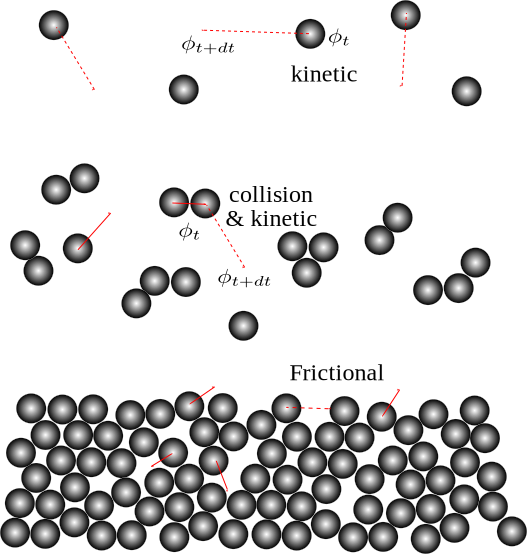
\includegraphics[width=0.95\textwidth]{kinetic}
\caption{The modes of viscous dissipation in a granular flow}
\label{fig:kinetic}
\end{figure}
%

For dense granular flow conditions, the total stress transmission in the flow 
regime is the sum of the rate-dependent (collision-transition) and the 
rate-independent (friction) components~\citep{Ng2008}. Addition of frictional 
stress component~\citep{Schaeffer1987} to the kinetic theory improves the 
ability of the model to predict the dense granular flows. The main advantage of 
kinetic theories is that they can be used to derive deterministic constitutive 
laws to describe the behaviour of granular flows in a theoretical 
framework~\citep{Jenkins1983}. Kinetic theories formulated on the assumption of 
solid phase stress as a viscous response have limitations when applied to 
granular flows. A viscous material produces no force unless it is in motion, 
hence the kinetic theory based on viscous solid phase cannot explain the static 
force exerted by the granular materials on the walls, as observed in 
experiments. The addition of a frictional component to the kinetic theory 
improves its prediction of granular flows. However, the frictional component 
that is based on long-duration contact is added to the instantaneous collision 
contact term. Also, the rapid-flow models based on gas kinetic theory assume 
that the molecular collisions are elastic, which means that they do not 
dissipate energy~\citep{Campbell2006}, which is in contrast to the reality. 
Finally, the important assumption of gas kinetic theory is molecular chaos, 
which assumes no correlation between the velocities or positions of the 
colliding particles, which is not true especially in a dense granular flow 
where the particles interact many times with their neighbours and a strong 
correlation between their velocities is inevitable.

\subsection{Shallow-water approximation}

Developing constitutive laws valid from the quasi-static to
dilute regimes remains a serious challenge. Simple 
elasto-plastic approach fails to model the collisional regimes in a granular 
flow. On the other hand, the original kinetic theory based 
on binary collisions does not capture the correct behaviour in the dense regime.
In configurations where the flowing layer is thin, a different theoretical 
framework is adopted.
%
%The Navier-Stokes equation in fluid mechanics is capable of describing the 
%dynamics of fluid flow under different conditions. However, the proposed 
%models 
%for granular flows tend to be specialized for a particular situation. By 
%drawing a simple analogy from fluid dynamics one can model granular flows as 
%non-Newtonian fluids using a variant of the Navier-Stokes equation;
One such approach is the depth-averaged shallow-water equation, which has been 
applied to solve granular flow dynamics with a reasonable amount of success. 
The Savage-Hutter model~\citep{Savage1991}, is a depth-average 
continuum-mechanics based approach which consists of hyperbolic partial 
differential equations to 
describe the distribution of the depth and the topography of an avalanching 
mass of cohesion-less granular media~\citep{Hutter2005}. This approach is based 
on the assumption that the horizontal length scale is very large in comparison 
with the vertical length scale, which allows us to neglect the horizontal 
partial derivatives relative to the vertical partial derivatives. Field 
observations of natural avalanches indicate an aspect ratio of $10^{-3} \mbox{ 
to } 10^{-4}$~\citep{Cawthor2006a}. By neglecting the vertical length 
scale, the continuum equation for conservation of mass and momentum can be 
written as
%
\begin{align}
 \partial_{\textit{x}}\textit{u}+\partial_{\textit{y}}\textit{v}& =0 \,,\\
 \partial_{\textit{t}}\textit{u}+\textit{u}\partial_{\textit{x}}\textit{u} + 
\textit{v}\partial_{\textit{y}}\textit{u} & =\left(\triangledown \cdot \sigma 
\right)_{\textit{x}} +\textit{\textbf{F}}_{\textit{x}} \,.
\end{align}
%
The continuum equation requires determining the components of the stress tensor 
and a suitable constitutive law. \textit{Savage-Hutter (SH) model} uses the 
Mohr-Coulomb law to describe the constitutive relation. The conservation of 
mass and momentum in the SH model is based on the assumption of granular flow 
as an incompressible fluid flow, which means that throughout the avalanche, the 
density of the avalanching material remains constant. 
Although~\citet{Hutter1995} observed the density of the granular flow to remain 
almost constant in a flow down a curved chute, the destructive nature of 
landslides and avalanches restricts us from inferring a conclusive result. The 
SH model involves the following assumptions: (1) Coulomb-type sliding takes 
place with a bed friction angle $\delta$, (2) Mohr-Coulomb frictional behaviour 
occurs inside the material with internal angle of friction, $\phi \ge \delta$, 
and (3) the velocity profile is assumed to be uniform throughout the avalanche 
depth. The granular flow over a rigid plane inclined at an angle, $\theta$ is 
shown in~\cref{fig:SH}. The mass and momentum balance in the SH model is 
written as
%
\begin{figure}[htbp]
\centering
\includegraphics[width=0.95\textwidth]{SH}
\caption{Illustration of the Savage-Hutter model}
\label{fig:SH}
\end{figure}
%
\begin{align}
&\frac{\partial \textit{H}}{\partial \textit{T}} + \frac{\partial}{\partial 
\textit{X}} (\textit{HU})  =  0 \,, \\
&\frac{\partial \textit{U}}{\partial \textit{T}} + \textit{U} \frac{\partial 
\textit{U}}{\partial \textit{X}}  = (\sin \theta - \tan \delta 
\textit{sgn}(\textit{U}) \cos \theta) -\beta \frac{\partial 
\textit{H}}{\partial \textit{X}} \,,
\end{align}
%
where capital letters denote non-dimensional quantities with respect to the 
typical horizontal and vertical length scales $(\textit{L}^{*},\textit{H}^{*})$ 
and the time scale $\sqrt{\textit{L}^{*}/\textit{g}}$. The key feature in the 
shallow water approximation is the Mohr-Coulomb constitutive law, which is 
applied at the free surface and at the base, to describe the granular flow. 
Comparison of the model with the post-calculation of Madlein avalanche in 
Austria indicates that the Coulomb basal friction is insufficient and requires 
an additional viscous component. The SH model's predictions were not 
satisfactory for granular flows down gentle slopes of inclination angle $\le 
30^{o}$, where granular materials exhibit premature stop~\citep{Hutter2005}. 
The SH model has not yet been tested in cases where the granular flow interacts 
with obstacles.

\subsection{Rheology}
\label{sec:muI}
Rheology is the science of flow of materials with solid and fluid 
characteristics. In practice, rheology is principally concerned with describing 
the mechanical behaviour of those materials that cannot be described by the 
classical theories, by establishing an empirical relation between deformation 
and stresses. Consider a granular assembly of grains having diameter 
\textit{d} and density $\rho_{\textit{d}}$ under a confining pressure 
\textit{P} (see~\cref{fig:rheology}). If the material is sheared at a 
constant shear rate, $\dot{\gamma} = \textit{V}_{\textit{w}} / \textit{L}$ is 
imposed by the relative movement of the top plate with a velocity $ 
\textit{V}_{\textit{w}}$. In the absence of gravity, the force balance implies 
that the shear stress, $\tau= \sigma_{\textit{xy}}$, and normal stress, 
$\textit{P}=\sigma_{\textit{xy}}$, are homogeneous across the cell. This 
configuration is the simplest configuration to study the rheology of granular 
flow, i.e. to study the effect of the strain rate, $\dot{\gamma}$, and 
pressure, \textit{P} on the volume and shear stress, $\tau$. 

Even though the granular materials have been extensively researched at 
microscopic level, the 
continuum representation of granular materials in terms of conservation of mass 
and momentum is still an area of concern~\citep{Midi2004,Daniel2007}. The 
prediction of rheology of granular materials even in the simplest case is 
complicated as they exhibit rate-dependent behaviour and no single constitutive 
equation is able to describe the behaviour over a range of shear stress 
rates.~\citet{DaCruz2005} developed a very famous rheology for granular flows, 
that is based on the simple two-dimensional shear in the absence of gravity and 
establishes that the flow regime and rheological parameters scale with a 
dimensionless number that represents the relative strength of inertia forces 
with respect to the confining pressure~\citep{Daniel2007}, along the lines 
of~\citet{Savage1991}. The shear stress, $\tau$, is proportional to the 
confining pressure, \textit{P}, and is written as
%
\begin{equation}
\tau = \textit{P} \mu (\textit{I}) \,.
\end{equation}
%
The friction coefficient $\mu$ depends on the single non-dimensional parameter 
\textit{I}, expressed as
\begin{equation}
\textit{I} = \frac{\dot{\gamma}d}{\sqrt{\textit{P}\rho_{\textit{p}}}} \,.
\end{equation}
%
The parameter \textit{I} can be interpreted in terms of different time scales 
controlling the grain flow. If the grains are rigid, i.e. neglecting the 
elastic properties of the grains, then \textit{I} is the only 
non-dimensional parameter in the problem. Hence, the shear stress, $\tau$, has 
to be proportional to the pressure, \textit{P}, times a function of \textit{I}. 
Comparing the shape of the function $\mu(\textit{I})$ with the experimental 
results of flow down an inclined plane,~\citet{Jop2006} observed that the 
frictional coefficient increases from a minimal value of $\mu_{\textit{s}}$ to 
an asymptotic value of $\mu_{2}$, when the value of \textit{I} increases. The 
variation of friction coefficient with \textit{I} is shown in~\cref{fig:mu}. 
The friction coefficient can be related to the inertial number \textit{I} as
%
\begin{equation}
\mu(I) = \mu_s + \frac{\mu_2 - \mu_s}{I_0/I+1}
\end{equation}
%
where $I_0$ is constant, typically in the range of 0.25 - 0.3. To formulate a 
complete constitutive model, it is essential to describe the volumetric 
behaviour. Based on the dimensional analysis, it can be argued that the volume 
change is also a function of dimensionless parameter \textit{I} and that it 
also depends on the maximum and the minimum possible void ratios and the time 
for microscopic rearrangement of grains. Consider two rows of mono-dispersed 
grains. When a grain is located on the gap formed by two adjacent grains, it is 
assumed to have a maximum packing fraction. As the grain is sheared along the 
bottom row of grains, it moves out of the gap resulting in 
a minimum packing fraction. The duration required for this rearrangement is 
directly proportional to the volume fraction. The dimensionless shear rate, 
expressed as the ratio between the duration of re-arrangement to the mean 
duration (see~\cref{fig:tmicro}), has a linear relationship with the volume 
fraction.

\begin{figure}[tbhp]
\centering
\includegraphics[width=0.95\textwidth]{Rheology}
\caption{Plane shear stress distribution under a constant pressure and shear 
rate for a granular assembly}
\label{fig:rheology}
\end{figure}

\begin{figure}[tbhp]
\centering
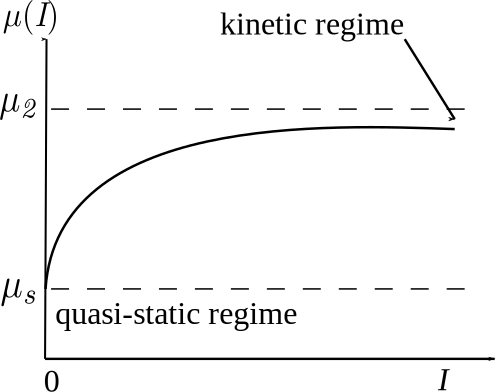
\includegraphics[width=0.95\textwidth]{mu}
\caption[Dependence of frictional coefficient $\mu$ with dimensionless shear 
rate $\textit{I}$]{Sketch of dependence of frictional coefficient $\mu$ with 
dimensionless shear rate $\textit{I}$, reproduced after ~\citet{Pouliquen2006}}
\label{fig:mu}
\end{figure}

In general, the flow regimes can be classified based on the dimensionless 
number \textit{I}~\citep{DaCruz2005}.~\Cref{fig:Regime} shows the variation of 
frictional coefficient $\mu$ and packing fraction $\phi$ with dimensionless 
number \textit{I} for different flow regimes under simple shearing. Dilute or 
``collisional'' flow occurs for \textit{I} $>10^{-1}$ and the grain collision 
is chiefly binary, accompanied  by additional ``bounce-back'' akin to 
gases~\citep{Kamrin2008}. In the dilute flow regime, the grains are rarely in 
long-duration contacts and can be described by dissipative Boltzmann kinetics. 
The ``quasi-static'' regime occurs at the other extreme of the spectrum, 
\textit{I} $<10^{-3}$, where the intermittent motion is prevalent. The inertial 
time is always small enough for the grains to align to a dense compaction, 
without significant collisional dissipation. The frictional sliding and 
stick-slip dynamics dominate the dissipation mechanism. The stress/strain-rate 
relationship becomes singular; driving the system with a range of quasi-static 
normalized shear rates all give the same time-average value for $\mu$. In this 
regime the dissipation is primarily frictional and rate-independent. Packing 
fraction appears independent of \textit{I}, and grain-level specifics are more 
important to flow dynamics. The moderate-flow regime is observed for \textit{I} 
between $10^{-3} \mbox{and }10^{-1}$, characterized by faster flows, with a 
high rate of contact formation and more energy dissipation per impact. In this 
regime, \textit{I} has a one-one relationship with $\mu$ and is large enough 
for rate dependence, but small enough for the flow to remain dense. Moderate 
flows also exhibit the property of \textit{shearing dilation}, where an 
increase in the normalized flow rate causes the steady-state packing fraction 
to decrease, which is different from \textit{shear dilation}, which refers to a 
decrease in the packing density as a function of total shear. Flows which are 
too slow to be moderate still undergo shear dilation due to geometric packing 
constraints, but shearing dilation occurs only in faster flows due to rate 
effects~\citep{Kamrin2008}. In moderate flows, the dissipation is primarily 
rate-sensitive due to energy loss during contact formation, yet packing remains 
dense

\begin{figure}[tbhp]
\centering
\includegraphics[width=0.95\textwidth]{Regime}
\caption[Variation of dimensionless parameter \textit{I} for different flow 
regimes]{Variation of dimensionless parameter \textit{I} for different 
flow regimes under simple shearing. (a) \textit{Quasi-static} ($I < 10^{-3}$): 
Dissipation is primarily frictional and rate-independent. Packing fraction 
appears independent of \textit{I}, and grain-level specifics are more important 
to flow dynamics; (b) \textit{Moderate} ($10^{-3} < I < 
10^{-1}$): the dissipation is primarily rate-sensitive due to energy loss 
during contact formation, yet packing remains dense; (c) \textit{Collisional} 
($I > 10^{-1}$): Flow becomes dilute and gas-like. Dynamics modelled best by 
dissipative Boltzmann kinetics. Redrawn after~\citep{Kamrin2008}}
\label{fig:Regime}
\end{figure}

\citet{Campbell2002} described the ``Moderate regime'' as an elastic granular 
flow regime, where the inter-grain stiffness governs the overall flow 
behaviour of the granular assembly. At high concentration, the stresses are 
proportional to the contact stiffness, and the streaming stiffness is 
negligible. When a dense granular assembly is sheared, the force chains that 
transmit the forces continue to rotate until it becomes unstable and collapses. 
As the force-chain rotates, the granular material tend to dilate, however it is 
restricted due to the constant volume constraint; instead, the rotation 
compresses the chain, generating an elastic 
response~\citep{Campbell2006}.~\citet{Campbell2002} divided the flow into the 
elastic and the inertial regimes. In the Elastic regime, the force is 
transmitted principally through the deformation of force chains with a natural 
stress scaling of $\tau \textit{d}/\textit{k}$. The force chain forms when the 
grains are sheared at the rate of $\dot{\gamma}$, and hence the rate of 
chain formation is proportional to the shear rate $\dot{\gamma}$. This 
transition regime can be explained using the force-chain concept. The lifetime 
of a force chain is proportional to $1/\dot{\gamma}$, consequently the product 
of rate of formation and the lifetime of the force chain is independent of 
$\dot{\gamma}$, and the stresses generated are quasi-static. However at higher 
shear rates, the elastic forces in the chain have to absorb the additional 
inertial force of the grains, requiring extra force to rotate the chain 
proportional to the shear rate. Even though the grains are locked in force 
chains, the forces generated must reflect the grain inertia. The ratio of 
elastic to inertial effects is governed by a dimensionless parameter
%
\begin{equation}
\textit{k}^{*} = \frac{k}{\rho \textit{d}^{3} \dot{\gamma}^{2}} \,,
\end{equation}
%
where ${k}/{\rho \textit{d}^{3} \dot{\gamma}^{2}}=({\tau}/{\rho \textit{d}^{2} 
{\gamma}^{2}})/(\tau\textit{d}/\textit{k})$ is the ratio of Bagnold's inertial 
to the elastic stress scaling. The important dimensionless parameter is 
$\textit{k}^{*}$, which is a measure of inertially-induced deformation, 
reflects the relative effects of elastic to inertial forces, i.e. at large 
$\textit{k}^{*}$, the elastic forces dominate and at small $\textit{k}^{*}$, 
inertial forces dominate~\citep{Campbell2006}. \citet{Campbell2002} observed a 
strong correlation between the coefficient of friction and the dimensionless 
parameter, \textit{k} as the flow progresses through different regimes, similar 
to the observation made by \citet{Kamrin2010}. 

Constitutive laws, which describe the dilatancy and friction, allow us to 
deduce the dependency of pressure and shear stress on shear rate and solid 
fraction. In contrast to the observation of \citet{Campbell2002}, 
\citet{DaCruz2005} found that the elastic stiffness has little effect on the 
constitutive law, for values greater than $10^{4}$, however that it does affect 
the coordination number.~\citet{DaCruz2005} also observed that the microscopic 
friction coefficient, $\mu$, has a significant influence on the dilatancy, and 
the solid fraction remains a linearly-decreasing function of \textit{I}. The 
frictional properties of the material are found to control the solid fraction, 
from the critical state to the collisional regime~\citep{DaCruz2005}. 

Although the rheology tends to describe the behaviour of granular flows, the 
mechanism of granular flows was found to vary with time, position and feedback 
mechanism~\citep{Iverson2003}. Rheology summarizes the mechanical behaviour at 
scales smaller in comparison with the Representative Elemental Volume (REV), 
for a substance modelled as a continuum. Rheology-based descriptions are 
generally restricted to homogeneous materials that exhibit time-independent 
behaviour, hence are unsuitable for describing granular flows where the stress 
history has a significant effect on the flow dynamics. The estimation of debris 
flow yield strength highlights the limitation of rheologies which do not 
consider the development of strength with evolution of time and 
space.~\citet{Johnson1965} emphasized that debris yield strength is 
predominantly a frictional phenomenon analogous to the Coulomb strength of 
granular soils, and that strength consequently varies with effective normal 
stress. Treatment of yield strength as an adjustable rheological property 
contradicts the basic understanding that the strength evolves as the 
debris-flow motion progresses. Frictional behaviour implies no explicit 
dependence of shear resistance on shear rate, whereas rheological formulas 
commonly used to model debris flows generally include a viscous component that 
specifies a fixed functional relationship between shear resistances and shear 
rate. Although rate-dependent shear resistance is observed in debris flows, its 
magnitude and origin indicate that it is ancillary rather than 
essential~\citep{Iverson2003}.

The two main modelling techniques that are commonly employed to describe the 
granular flow are the continuum approach and the discrete element approach. The 
continuum approach involves treating granular assembly as a continuum and 
describing its response using constitutive laws, while the discrete approach 
involves considering the individual grains of the granular material and 
applying Newton's laws of motion to describe the deformation of the granular 
material. These approaches are adopted in the present study and detailed 
discussions are provided in~\cref{chapter:numerical_modelling}. 

\section{Studies on granular flows}
The flow of dense granular material is a common phenomenon in engineering 
predictions, such as avalanche, landslides, and debris-flow modelling. Despite 
the huge amount of research that has gone into describing the behaviour of 
granular flow, a constitutive equation that describes the overall behaviour of 
a flowing granular material is still lacking. To circumvent this difficulty, 
depth-averaged constitutive equations have been employed along with an 
empirical friction coefficient and a velocity profile deduced from 
experiments~\citep{Midi2004,Iverson2003,Pouliquen1999}. Although this approach 
has been successful to a certain extent in predicting geophysical 
flows~\citep{Pouliquen2002a, Hutter1995}, it presents two important 
shortcomings~\citep{Lajeunesse2005}: first, the depth-average method is true 
only if the thickness of the flowing layer is thin in comparison with the 
lateral dimension, and second, the empirical laws are deduced from experiments 
performed under steady-flow conditions. These cast doubts on the validity of 
the depth-averaged approach. Two simple granular flow studies, granular column 
collapse and granular flow down an inclined plane, have been carried out by 
various researchers to understand the flow behaviour.

\subsection{Granular column collapse}
\citet{Lube2005} and ~\citet{Lajeunesse2004} have carried out experimental 
investigation on the collapse behaviour of a granular column on a horizontal 
plane. Both the experiments involved filling a cylinder of height 
$\textit{H}_{\textit{0}}$ and radius $\textit{L}_{\textit{0}}$ with granular 
material of mass \textit{m}. ~\Cref{fig:exp} 
shows the schematic view of the experimental configuration of a 2-D granular 
column collapse in a rectangular channel. The granular column is then released 
\textit{en masse} by quickly removing the cylinder, thus allowing the granular 
material to collapse onto the horizontal surface, forming a deposit having a 
final height 
$\textit{H}_{\textit{f}}$ and radius $\textit{L}_{\textit{f}}$. Although the 
experiment is simple and attractive allowing us to explore the limitations of 
depth-average modelling techniques, a constitutive law that could describe the 
entire flow behaviour is still lacking. The primary aim of these experiments 
was to determine the scaling laws for the run-out distance.


\begin{figure}[tbhp]
\centering
\includegraphics[width=0.85\textwidth]{experiment_setup}
\caption{Schematic view of the experimental configuration of a 2-D collapse in 
a rectangular channel~\citep{Lajeunesse2004}}
\label{fig:exp}
\end{figure}

\subsubsection{Deposit morphology}
\citet{Lajeunesse2005} observed that the flow dynamics and the final deposit 
remain independent of the volume of granular material that is released, but 
depend only on the initial aspect ratio \textit{a} of the granular column. 
The experiment was carried out to understand the effect of the geometrical 
configuration on the run-out, the mechanism of initiation of the flow, the 
evolution of flow with time, and to understand how such complex flow dynamics 
could produce deposits obeying simple power laws.~\citet{Lube2005} explored the 
effect of density and shape of grains on flow dynamics, 
whereas~\citet{Lajeunesse2004} worked with glass beads to study the influence 
of bead size and substrate properties on the deposit morphology. Surprisingly, 
both drew the striking conclusion that the flow duration, the spreading 
velocity, the final extent of the deposit, and the fraction of energy 
dissipated during the flow can be scaled in a quantitative way independent of 
substrate properties, bead size, density, and shape of the granular material 
and released mass, \textit{m}~\citep{Lajeunesse2005}.

The normalised final run-out distance as a function of the initial aspect 
ratios of the granular column under plane-strain and axi-symmetric conditions 
is shown in~\cref{fig:Runout_Exp}.~\citet{Lube2005} scaled the run-out distance 
as
\begin{align}
& \frac{\textit{L}_{\textit{f}}- 
\textit{L}_{\textit{0}}}{\textit{L}_{\textit{0}}} \approx
\begin{cases} 
1.24\textit{a}, \qquad &\textit{a} \lesssim 1.7 \\
1.6\textit{a}^{1.2}, \qquad &\textit{a} \gtrsim 1.7
\end{cases}
\end{align}
while~\citet{Lajeunesse2005} scaled run-out as
\begin{align}
& \frac{\textit{L}_{\textit{f}}- 
\textit{L}_{\textit{0}}}{\textit{L}_{\textit{0}}} \approx
\begin{cases} 
1.35\textit{a}, \qquad &\textit{a} \lesssim 0.74 \\
2.0\textit{a}^{1.2}, \qquad &\textit{a} \gtrsim 0.74
\end{cases}
\end{align} 

The normalised final height as a function of the initial aspect ratios of 
the granular column under plane-strain and axi-symmetric conditions is 
shown in~\cref{fig:Height_Exp}. The evolution of the scaled deposit height 
$\textit{H}_{\textit{f}}/\textit{L}_{\textit{0}}$ with the aspect ratio 
\textit{a} for axis-symmetric collapse~\citep{Lajeunesse2005} is given as 
\begin{align}
\textit{H}_{\textit{f}}/\textit{L}_{\textit{0}} \approx 
\begin{cases}
\textit{a}, \qquad &\textit{a}\lesssim 0.74 \\
0.74, \qquad &\textit{a}\gtrsim 0.74
\end{cases}
\end{align}
and for two-dimensional collapse
\begin{align}
\textit{H}_{\textit{f}}/\textit{L}_{\textit{0}} \approx 
\begin{cases}
\textit{a}, \qquad &\textit{a}\lesssim 0.7 \\
\textit{a}^{1/3}, \qquad &\textit{a}\gtrsim 0.7
\end{cases}
\end{align}

\begin{figure}[tbhp]
\centering
	\begin{subfigure}[b]{0.85\textwidth}
	\centering
	\includegraphics[width=\textwidth]{Runout_Exp}
	\caption{Normalised final run-out distance vs aspect ratio}
	\label{fig:Runout_Exp}
	\end{subfigure} \\

	\begin{subfigure}[b]{0.85\textwidth}
	\centering
	\includegraphics[width=\textwidth]{Height_Exp}
	\caption{Normalised height vs aspect ratio}
	\label{fig:Height_Exp}
	\end{subfigure}
	\label{fig:Run_Height_Exp}
	\caption[Normalised final run-out and height as a function of initial aspect ratio for 
	plane-strain and axi-symmetric collapse]{The normalised final run-out distance and final height 
	as a function of the initial aspect ratios of the granular column under plane-strain 
	and axi-symmetric conditions~\citep{Lajeunesse2004}.}
\end{figure}


Quasi-two-dimensional collapse of a granular column on a horizontal 
surface~\citep{Lajeunesse2005} reveals that the geometric configuration 
influences the scaling of the run-out distance. The run-out in a 
quasi-two-dimensional collapse of a granular column in a rectangular channel, 
is scaled as 
\begin{align}
& \frac{\textit{L}_{\textit{f}}- 
\textit{L}_{\textit{0}}}{\textit{L}_{\textit{0}}} \approx
\begin{cases} 
1.2\textit{a}, \qquad &\textit{a} \lesssim 2.3 \\
1.9\textit{a}^{2/3}, \qquad &\textit{a} \gtrsim 2.3
\end{cases}
\end{align} 
At large aspect ratios, the run-out is well represented by a simple power-law 
dependence. The exponent is found to vary with the channel width: $\Delta 
\textit{L}/\textit{L}_{\textit{0}} \approx \lambda \textit{a}^{0.65}$ for 
narrow channels and $\Delta \textit{L}/\textit{L}_{\textit{0}} \approx \lambda 
\textit{a}^{0.9}$ for wide channels. The constant of proportionality $\lambda$ 
is found to vary with the internal friction angle of the granular material, 
which contradicts the findings of previous authors, especially~\citet{Lube2005} 
who found that the scaling of run-out is independent of the granular material, 
perhaps due to a narrow range of experimental materials~\citep{Staron2005}.
~\citet{Balmforth2005} observed that the material properties have almost no 
influence on the exponent of the normalised run-out as a function of the 
initial aspect ratio. The numerical constant of proportionality, however, 
showed clear material dependence. This corroborates the conclusions 
of~\citet{Lajeunesse2004} and refutes that 
of~\citet{Lube2005}.~\citet{Daerr1999} also observed strong influence of 
initial packing density and the internal structure on the behaviour of 
granular flows. 


The scaling found for quasi-two-dimensional experiments in the narrow gap 
configuration gives similar results as~\citet{Lube2005} and roughly a scaling 
of $\textit{L}_{\textit{f}}/({\textit{L}_{\textit{f}} - 
\textit{L}_{\textit{0}}}) \propto \textit{a}^{2/3}$. Numerical simulations of 
granular column collapse by~\citet{Zenit2005} and~\citet{Staron2005} yielded 
similar scaling of run-out with aspect ratio \textit{a}, unlike other 
authors,~\citet{Zenit2005} did not observe any transition in the run-out 
behaviour of a granular column collapse with the aspect ratio \textit{a}. The 
origin of the exponents is still under discussion. No model has yet achieved a 
comprehensive explanation of the dependence of the complex-collapse dynamics on 
simple power laws. However, it was observed that a simple friction model cannot 
effectively describe the collapse dynamics.~\citet{Staron2005} explained the 
mechanism of spreading using an initial potential energy approach. 

For higher 
aspect ratios, the free fall of the column controls the dynamics of the 
collapse and the energy dissipation at the base is attributed to the 
coefficient of restitution. Thus, the initial potential energy stored in the 
system is dissipated by sideways flow of material and the mass ejected sideways 
is found to play a significant role in the spreading process, i.e. as 
\textit{a} increases, the same fraction of initial potential energy drives an 
increasing proportion of initial mass against friction, thus explaining the 
power-law dependence of the run-out distance on \textit{a}. Taking advantage 
of the similarity between granular slumping and the classical ``\textit{dam 
break}'' problem in fluid mechanics,~\citet{Kerswell2005} solved both the 
axis-symmetric and two-dimensional granular-collapse problem using the 
shallow-water approximation. Although the results of the shallow-water 
approximation have good agreement with experimental results, the shallow-water 
approximation overestimates the run-out distance for columns with aspect ratio 
\textit{a} greater than unity. The shallow-water equation does not take into 
account the effect of vertical acceleration~\citep{Lajeunesse2005}, which has 
been found to play a significant role in controlling the collapse 
dynamics~\citet{Staron2005}, thus resulting in overestimation of run-out. Tall 
columns showed significantly longer run-out distances when continuum approaches 
like material point method is used~\citep{Bandara2013,Mast2014}.

The scaling of the final collapse height is 
found to be similar with the 
experimental results of~\citet{Lube2005} and~\citet{Balmforth2005}, and the 
numerical simulation of~\citet{Staron2005}. Numerical simulation of granular 
column collapse~\citep{Lacaze2008,Staron2005} showed a transition in the flow 
behaviour at \textit{a}$\ge 10$, which was not observed in granular collapse 
experiments~\citep{Balmforth2005,Lube2005,Lajeunesse2004}. In the 
depth-averaged shallow-water model, which integrates over the depth, the 
emphasis was on capturing the scaling of the final deposit, rather than trying 
to reproduce the internal structure of the flow. The shallow-water model 
captures well the final deposit scaling for lower aspect ratios, however fails 
to capture the flow dynamics for granular columns with higher aspect ratios, 
where the flow is governed mainly by the vertical collapse of the granular 
column as a whole. The run-out distance predicted is clearly erroneous in the 
collapse regime where there is a sudden drop in efficiency by which the initial 
potential energy of the system is converted into the kinetic energy for 
spreading. Even a more sophisticated basal drag law will not be sufficient to 
model the mechanism of granular column collapse realistically using the 
shallow-water approximation~\citep{Kerswell2005}.




\subsubsection{Flow dynamics}
The variation of final scaled deposit with aspect ratio \textit{a} shows a 
transition in the run-out behaviour for an aspect ratio of 1.7, indicating a 
transformation in the spreading process or the collapse mechanism. To 
understand the collapse mechanism, it is insufficient to study only the final 
scaled profile, and hence the entire flow process should be 
analysed.~\citet{Lajeunesse2005} observed the flow regime and deposit 
morphology for a quasi-two-dimensional granular collapse in a rectangular 
channel. The flow phenomenology of a granular column collapse in a rectangular 
channel was surprisingly similar to that observed in the axis-symmetric 
collapse~\citep{Lube2005,Lajeunesse2004}, depending mainly on the initial 
aspect ratio \textit{a}. 

The flow dynamics involve spreading of granular mass 
by avalanching of flanks producing a truncated cone for \textit{a} $\lesssim 
0.74$ and a cone for \textit{a} $\gtrsim 0.74$; the transition of flow dynamics 
occurs as the value of \textit{a} is increased. The evolution of the deposit 
height remains independent of the flow for \textit{a} $\lesssim 0.7$, however 
it exhibits significant dependence on the geometrical configuration for 
\textit{a} $\gtrsim 0.7$. In rectangular channels, the effect of side-wall on 
the run-out behaviour was observed; the surface velocity profile between the 
side walls is that of a plug flow with a high slip velocity at the wall and low 
shear along the direction transverse to the flow. Systematic measurements 
indicate that the ratio of the maximum surface velocity to the surface velocity 
at the wall is between 1.2 and 1.4.~\citet{Lajeunesse2005} observed that the 
difference between the evolution of $\textit{H}_{\textit{f}}$ in the 
axis-symmetric geometry and in the rectangular channel is not an experimental 
artefact due to the side wall friction, but is a \textit{geometrical effect}. 


Understanding the internal flow structure will provide an insight into the 
complex collapse dynamics. For smaller values of aspect ratio \textit{a} $\le 
0.7$, the flow is initiated by a failure at the edge of the pile along a 
well-defined fracture surface above which material slides down and below which 
the grains remain static. The grains located above the fracture move 
``\textit{en masse}'' and most of the shear is concentrated along this surface 
forming a ``\textit{truncated-cone-like}'' deposit with a central motionless 
plateau. For columns with larger aspect ratios, the flow is still initiated by 
failure along a well-defined surface, an inclined plane in two-dimensional 
geometry or a cone in the axis-symmetric case. However, the initial height of 
the column is much higher than the top of the failure surface, causing a 
vertical fall of grains until they reach the summit where they diverge along 
the horizontal direction, dissipating a lot of kinetic energy, resulting in a 
final conical deposit. Interestingly, the final deposit height coincides with 
the summit of the failure surface in the axis-symmetric geometry, whereas in 
the rectangular channel, the deposit summit always lies above the top of the 
failure surface~\citep{Lajeunesse2005}. The evolution of failure surface at $t 
= 0.4 \tau_c$ for granular columns with initial aspect ratio of 0.4 and 3 are 
shown in~\cref{fig:Deposit}.

\begin{figure}[tbhp]
\centering
\includegraphics[width=0.975\textwidth]{Deposit}
\caption{The extent of the failure surface for granular columns with initial 
aspect ratio of 0.4 and 3 at time $t= 0.4\tau_c$~\citep{Lajeunesse2004}. Short 
columns show truncated conical deposit at the end of the flow, while tall 
columns exhibit conical deposit.}
\label{fig:Deposit}
\end{figure}


Identification of the static region is an important task, as it is a prime 
component in describing the collapse mechanism. Regardless of the experimental 
configuration, for all values of \textit{a} the flow is initiated by rupture 
along a well-defined failure surface and the failure angle remains of the order 
of $50^{o} \mbox{ to } 55^{o}$. The failure angle is consistent with an 
interpretation of \textit{active Coulomb failure}, which leads to a failure 
angle $\phi_{\textit{f}}=45^{o}+\delta / 2$, where $\delta$ is the internal 
friction angle of the granular material. Estimating the internal friction angle 
of glass beads from the angle of repose as $22^{o}$, the failure angle is 
estimated as $56^{o}$, which is in good agreement with the experimental 
findings. Contrary to the suggestion of~\citet{Lajeunesse2004}, the fracture 
angle was found to have no direct effect on the transition between truncated 
cone and conical deposit occurring at aspect ratio \textit{a} of 
0.7~\citep{Lajeunesse2005}.~\citet{Schaeffer1990} observed the onset of 
instability, when the neutrally stable plane waves makes an angle of 
$\phi_{\textit{I}}$ with the major principle stress axis. The onset of 
instability triggers unstable plane waves in a narrow wedge of $56^{o}\mbox{ to 
}65^{o}$, which corresponds to the angle of shear bands: this observation 
matches well with the failure angle observed in the granular flow. A 
rate-dependent constitutive relationship~\citep{Jop2006} for dense granular 
flows indicates the angle of shear-band orientation depends on the inertial 
number \textit{I}. For small to moderate values of \textit{I}, the orientation 
of shear bands is found to vary from the Roscoe and the Coulomb solutions to a 
unique admissible angle~\citep{Lemiale2011}.~\citet{Daerr1999} observed active 
Coulomb-type yielding in transient surface flows for granular materials having 
a packing density of 0.62 to 0.65. The comparison of initial and final areas 
indicates a change in the packing; the initial area is systematically smaller 
than the final area. This change in packing is typical of granular slumping in 
a channel and reflects that the pile, which initially had a relatively close 
packing, expanded (by about 10\%) as the flow progressed, to form the final 
deposit~\citep{Balmforth2005}.

A critical time $\tau_{\textit{c}}$ is defined as the transition time at which 
the flow is fully developed. The velocity field then depends on the position of 
grains along the pile, see~\citet{Lajeunesse2005}. In the front, the flow 
involves the entire thickness of the pile and corresponds to a plug flow in the 
horizontal direction. In the region above the static core, the flow is locally 
parallel to the failure surface and has an upper linear part and a lower 
exponential tail near the static bed~\citep{Lajeunesse2005}. The velocity flow 
profile is similar to that of a steady granular flow~\citep{Midi2004}. As the 
pile spreads, interface separation occurs as the flow diverges and the static 
region starts to move inwards; this effect is predominant in the case of 
granular flows in a rectangular channel. The typical velocity observed at the 
front of the ejecting mass is 
$\textit{v}=\sqrt{2\textit{g}\textit{L}_{\textit{0}}}$. 

The flow evolution as per~\citet{Staron2005} involves three stages. The first 
stage involves conversion of the initial potential energy of the grains into 
vertical motion, resulting in downwards acceleration of grains. In the second 
stage, the grains undergo collision with the base and/or neighbouring grains, 
and their vertical motion is converted into horizontal motion. In the final 
stage, the grains eventually leave the base area of the column and flow 
sideways. The typical time required for the flow to cease and form the final 
deposit, from the instant of its release, is 
$\textit{T}=\sqrt{2\textit{H}_{\textit{0}}/\textit{g}}$~\citep{Staron2005}. 
While plotting the variation of normalized potential and kinetic energy with 
normalized time,~\citet{Staron2005} observed that the flow ceases when the 
normalized time $\textit{t}/\textit{T}_0$ is 2.5, i.e. the flow is assumed to 
have stopped when the total normalized energy is almost zero. This observation 
is consistent with the experimental results of~\citet{Lube2005} 
and~\citet{Lajeunesse2005}. The transition of the flow occurs when the 
normalized time $\textit{t}/\textit{T}_0$ is 1.0 or at critical time 
$\tau_{\textit{c}}$, which is defined as the time at which the flow is fully 
mobilized.

\subsubsection{Comments on modelling}

In order to have a detailed understanding of the final profile of the collapsed 
granular column, it is important to solve the collapse problem as an 
\textit{initial-value problem}~\citep{Balmforth2005}, beginning from the 
instant of release and extending to the time when the material finally ceases 
to flow, forming the final deposit. As the process of granular collapse 
involves collective dynamics of collisions and momentum transfer, the 
prediction of the trajectory of a single grain is difficult. In fact, there are 
quantitative disagreements between theory and experiments; the final shapes are 
reproducible, but not perfectly. Some of the disagreement arises because the 
experiments did not have exactly the same amount of materials; it is indeed 
difficult to fill the pile with exactly the same amount of material, which 
results in differences in packing. However, the theoretical errors are due to 
the incapability of the models to capture the physics that governs the flow 
dynamics~\citep{Balmforth2005}. Shallow water models fail to account for the 
vertical acceleration, which is responsible for the momentum transfer and, in 
turn, the spreading process. This restricts the shallow water model to capture 
the mechanism of collapse until the critical time $\tau_{\textit{c}}$. 
Surprisingly, shallow-water models capture certain experimental aspects for 
columns with lower aspect 
ratios~\citep{Mangeney2010,Balmforth2005,Kerswell2005}, even though the 
contrast between surface flows and the static region is important in this range 
of aspect ratio. Thus, the assumption of plug flow in the horizontal direction 
is not critical in capturing the run-out behaviour, especially if the basal 
friction coefficient is used as a fitting parameter~\citep{Lajeunesse2005}. 

Simple mathematical models based on conservation of horizontal momentum capture 
the scaling laws of the final deposit, however they fail to describe the 
initial transition regime, indicating that the initial transition has 
negligible effect on the run-out, which is incorrect. Models based on the 
initial potential energy show promise, but the effect of material properties, 
such as basal friction and coefficient of restitution, on the run-out behaviour 
is still unclear and produces non-physical run-outs. The famous 
$\mu(\textit{I})$ rheology predicts well the normalized run-out behaviour in 
comparison with the experimental results, for lower aspect ratios. The 
spreading dynamics is found to be similar for the continuum and grain 
approaches; however, the rheology falls short in predicting the run-out 
distance for higher aspect ratios. Unlike~\citet{Lube2005}, many 
researchers~\citep{Balmforth2005,Kerswell2005} observed strong dependency of 
material properties on the run-out distance, moistening the materials or the 
sides of the channel even by a small amount leads to markedly different 
results.~\citet{Staron2007a} observed that the friction has little effect on 
the 
run-out for granular column collapse for high aspect ratios, which are driven 
mainly by the free vertical fall of grains. The initial conditions have a 
significant impact on the overall behaviour of the granular system, indicating 
the significance of the triggering mechanism in case of the natural 
flows~\citep{Staron2007a}. Numerical investigations, such as Discrete Element 
Method 
techniques, allow us to evaluate quantities which are not accessible 
experimentally, thus providing useful insight into the flow dynamics. 
Subsequent chapters discuss the methodology and modelling of granular column by 
continuum- and discrete-element approaches.

\subsection{Flow down an inclined plane}
Studies on the flow of granular materials down inclined planes are important to 
understand the mechanism of geophysical hazards, such as granular avalanches, 
debris flows and submarine landslides. Large scale field tests on dry and 
saturated granular materials were carried out to capture the mechanism of 
granular flows down an inclined plane~\citep{Okada2008,Denlinger2001}. The 
granular material stored in a reservoir at the top of the inclined plane is 
released by opening a gate; the material flows down and develops into a dense 
granular flow. 

A variant of the above experiment is the experiment on fluidised beds 
which involves an initial bed of granular material of thickness `\textit{h}' 
which is inclined gradually until the granular material flows. When the plane 
inclination reaches a critical angle, $\theta_{\textit{start}}$, the material 
starts to flow and reaches a sustained flow until the inclination is decreased 
down to a second critical angle, $\theta_{\textit{stop}}$~\citep{Midi2004}. The 
occurrence of two critical angles indicates the hysteretic nature of granular 
materials. Reciprocally, the critical angle thresholds can be interpreted in 
terms of critical layer thickness $\textit{h}_{\textit{stop}}(\theta)$ and 
$\textit{h}_{\textit{start}}(\theta)$. The measurement of  
$\textit{h}_{\textit{stop}}(\phi)$ is easier as it corresponds to the thickness 
of the deposit remaining on the plane once the flow has ceased. 

\begin{figure}[tbhp]
\centering
\includegraphics[width=0.85\textwidth]{Incline}
\caption{Rough inclined plane: (a) Set-up, and (b) $h_{stop}(\theta)$ (black 
symbols) and $h_{start}(\theta)$ (white symbols). Reproduced 
after~\citet{Midi2004}.}
\label{fig:Incline}
\end{figure}


Three regions can be observed: a region where no flow occurs, 
$(\textit{h}<\textit{h}_{\textit{stop}}(\theta))$, a sub-critical region where 
both static and flowing layers can exist $(\textit{h}_{\textit{stop}}(\theta) < 
\textit{h} < \textit{h}_{\textit{start}}(\theta)$ and a region where flow 
always occurs, $(\textit{h}>\textit{h}_{\textit{start}}(\theta))$. In the flow 
regime, i.e. $(\textit{h}>\textit{h}_{\textit{start}}(\theta))$, the flow is 
steady and uniform for moderate inclination, but accelerates along the plane 
for large inclinations~\citep{Midi2004}. The critical angle controlling the 
flow behaviour tends to increase when the thickness of the bed 
decreases~\citep{Pouliquen2002a,Daerr1999}, which can be attributed to the 
non-trivial finite-size effects and/or boundary effects that are not well 
understood~\citep{Forterre2008}. 

Fast moving granular flows can undergo a motion-induced self-fluidisation 
process under the combined effects of front instabilities setting on at large 
values of the Froude number which are responsible for extensive air 
entrainment, and small deflation rates associated with small incipient 
fluidisation velocities and longer collapse time of the bed solids. 
Self-fluidisation results in enhanced mobility of the solids, causing an 
inviscid flow to an extent that may largely exceed the establishment of a 
``\textit{granular liquid}'' state in purely granular 
flow~\citep{Bareschino2008}. It is understood that, for a granular material to 
flow, it has to exceed a certain critical threshold, i.e. the friction 
criterion: the ratio of shear stress to normal stress. As there is no internal 
stress scale for a granular material, granular materials exhibit solid-fluid 
transition behaviour based on the friction criterion~\citep{Forterre2008}. The 
stress ratio in the flowing regime above the static bed indicates the 
solid-to-fluid transition is a yielding phenomenon and can be described by 
Mohr-Coulomb-like failure criterion~\citep{Zhang1992}. This is in contrast to 
the mechanism of behaviour of other complex fluids, where there is an internal 
stress scale linked to the breakage of microscopic structure. From a 
microscopic point of view, the strength of the granular materials is due to the 
internal friction between grains, but packed frictionless materials still 
exhibit macroscopic friction.

Constitutive laws based on Plasticity-theories relate the micro-structure to 
the macroscopic behaviour~\citep{Roux2002}, which provide useful insight into 
the mechanism of granular flow. However, at present they are limited to 
initiation of deformation and do not predict the quasi-static flow. Material 
Point Method simulation of granular flow down an inclined 
plane~\citep{Abe2006,Bandara2013} captures the flow behaviour in the initial 
stages, however it exhibits inconsistent behaviour when the granular material 
ceases to flow. This may be due to the application of small deformation theory 
to a large deformation problem and to the use of zero dilation. In the case of 
flow down an inclined plane, the only control parameter is the flow rate, 
\textit{Q}, and uniform, steady flows are possible if the system is confined 
between walls. The additional friction induced by the lateral walls has a 
significant effect on the flow and causes localization at the free surface. The 
$\mu(\textit{I})$ friction law captures the velocity profile and the 
localization at the free surface. However, the model fails to capture the 
transition from a continuous flow to an avalanching regime as the flow rate is 
decreased~\citep{Pouliquen2006}. The flow can cause strong Coulomb shear 
stresses to develop on a plane normal to the basal flow boundary. The stresses 
dissipate energy as the flow encounters obstructions: models that lack 
multi-dimensional momentum transport or Coulomb friction cannot represent this 
energy dissipation and lodging. 

\subsection{Saturated and submerged granular flows}
Geophysical hazards, such as debris flows and submarine landslides, usually 
involve flow of granular solids and water as a single-phase system. The 
momentum transfer between the discrete and the continuous phases significantly 
affects the dynamics of the flow as a whole~\citep{Topin2011}. Although certain 
macroscopic models are able to capture simple mechanical 
behaviours~\citep{Peker2007}, the complex physical mechanisms occurring at the 
grain scale, such as hydrodynamic instabilities, formation of clusters, 
collapse, and transport~\citep{Topin2011}, have largely been ignored. In 
particular, when the solid phase reaches a high volume fraction, the strong 
heterogeneity arising from the contact forces between the grains, and the 
hydrodynamic forces, are difficult to integrate into the homogenization process 
involving global averages~\citep{Topin2011}. 

In two-phase models~\citep{Pitman2005}, the momentum transfer between the 
grains and the suspension fluid depends on the momentum equations of both 
the phases. In case of mixture theory based models~\citep{Meruane2010}, the 
shear-induced migration 
and grains collisions are considered in an average sense. In order to 
describe the mechanism of saturated and/or immersed granular flows, it is 
important to consider both the dynamics of the solid phase and the role of the 
ambient fluid~\citep{Denlinger2001,Iverson1997}. The dynamics of the solid 
phase alone are insufficient to describe the mechanism of granular flow in a 
fluid; it is important to consider the effect of hydrodynamic forces that 
reduce the weight of the solids inducing a transition from dense-compacted to 
dense-suspended flows, and the drag interactions which counteract the movement 
of the solids~\citep{Meruane2010}.


\citet{Iverson2000} observed in the 
large-scale field tests that the soil prepared in a loose state on a slope and 
subjected to a rainfall flows rapidly like a liquid when it breaks, whereas a 
dense soil only slowly creeps. The underlying mechanism is related
to the dilation or contraction character of the granular material, which the 
authors described as the ``pore pressure feedback''. The compaction or dilation 
of grains can cause additional stress in the grains which can stabilise or 
destabilise the soil. The flow is controlled by the coupling between the 
dilatancy of the granular layer and the development of pore pressure in the 
fluid phase~\citep{Pailha2008}.

The collapse of a granular column, which mimics the collapse of a cliff, has 
been extensively studied in the case of dry granular material, when the 
interstitial fluid plays no role. The case of the collapse in presence of an 
interstitial fluid has been less studied~\citep{Topin2012}. 
\citet{Rondon2011} performed granular column collapse experiments in fluid to 
understand the role of initial volume fraction. The experimental set-up 
of granular collapse in fluid performed by~\citet{Rondon2011} is shown 
in~\cref{fig:Fluid_Collapse}.

\begin{figure}[htbp]
\centering
\includegraphics[width=0.65\textwidth]{Fluid_Collapse}
\caption{Experimental set-up of granular collapse in fluid~\citep{Rondon2011}.}
\label{fig:Fluid_Collapse}
\end{figure}

They observed that, contrary to 
the dense case, the whole loose column is mobilised immediately. The loose 
column in fluid spreads almost twice than the dense case. The 
collapse of a granular column in a viscous fluid is found to be mainly 
controlled by the initial volume fraction and not by the aspect ratio of the 
column. The role of the initial volume fraction observed in the viscous 
collapse can be understood by the pore pressure feedback mechanism proposed 
by~\citep{Schaeffer2008,Iverson2000} in the context of landslides. The dense 
column needs to dilate in order to flow. When it starts to fall, liquid
is then sucked into the column, which is then stabilized by the additional 
viscous drag~\citep{Rondon2011,Topin2012}. By opposition the loose column when 
it starts flowing expands and ejects liquid, leading to a partial fluidisation 
of the material (\cref{fig:Runout_PWP_Fluid_Exp}). 

\begin{figure}[htbp]
\centering
\includegraphics[width=0.85\textwidth]{Runout_PWP_Fluid_Exp}
\caption{Evolution of run-out and pore-water pressure at the bottom for 
granular column collapse in fluid for dense and loose 
conditions~\citep{Rondon2011}.}
\label{fig:Runout_PWP_Fluid_Exp}
\end{figure}

In the dry case, inertia is 
responsible for the enhance of mobility at high aspect ratio. In the viscous 
regime, the inertial effects 
remain negligible, which could explain why the important parameter controlling 
the dynamics is the initial volume fraction and not the initial aspect 
ratio.~\citet{Topin2011} observed that the run-out exhibit a power-law relation 
with the peak kinetic energy and the largest value of run-out in fluid inertial 
regime, and the lowest in grain-inertial and intermediate value for the 
viscous-regime. The viscous regime is where the grain reaches the viscous 
limit velocity, the Stoke's number $S_t << 1$ and the density ratio $r >> 
S_t$~\citep{CourrechDuPont2003}. However, the role of the volume fraction on 
dry granular collapse has not been precisely studied and the preparation of the 
pile may also play a role~\citet{Daerr1999a}.

\citet{Cassar2005} carried out experimental 
investigation on the flow of dense granular material down an inclined plane 
fully-immersed in water. The velocities observed in the submarine case were 
found to be a magnitude smaller than the dry condition. The run-out behaviour 
collapse on to a single friction law, which shows that the major role of the 
fluid is to change the time it takes for a grain to fall into a void-space. 
The $\mu(\textit{I})$ rheology for dry dense flows captures the behaviour of 
dense submarine granular flows, if the inertial time scale in the rheology is 
replaced with a viscous time scale. In the case of dry granular flows, the 
parameter \textit{I} is defined as the ratio between the time taken for a 
grain to fall into the hole, $\textit{t}_{\textit{micro}}$, and the 
meantime, $\textit{t}_{\textit{mean}}$, which is inversely related to the shear 
rate.~\citet{Pitman2005} observed that if the fluid inertial effects are small 
enough, then a simpler model can be adopted. Sketch of the motion of a grain 
z(t) during a simple shear $\dot{\gamma}$ under a confining pressure $P_g$ is 
shown in~\cref{fig:tmicro}. Hence, assuming that the fluid 
velocity is low enough for the contact interaction between grains to be 
significant, the time taken by the grain to fall into a hole, 
$\textit{t}_{\textit{micro}}$, is  then controlled by the viscosity of the 
ambient fluid. Thus, the dimensionless parameter can be modified to incorporate 
the viscous time to describe granular flow in a fluid~\citep{Pouliquen2005}. 

\begin{figure}[htbp]
\centering
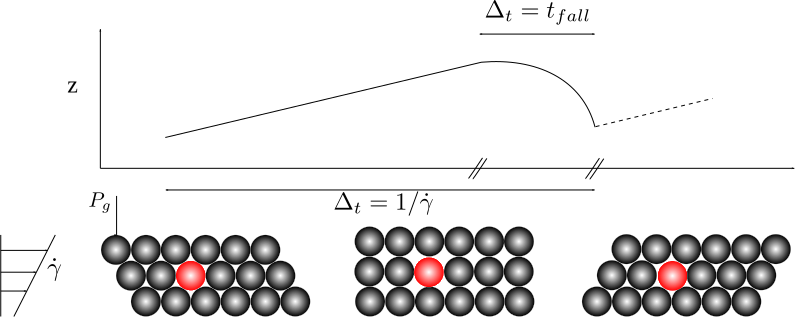
\includegraphics[width=0.85\textwidth]{tmicro}
\caption{Sketch of the motion of a grain z(t) during a simple shear 
$\dot{\gamma}$ under a confining pressure $P_g$.}
\label{fig:tmicro}
\end{figure}


The constitutive law is found to be valid only for the steady uniform regime; 
unsteady phenomena such as the triggering of avalanches result in coupling 
between the granular grains and the ambient fluid and are much more complex 
to model. Transient regimes characterized by change in solid fraction, dilation 
at the onset of flow and development of excess pore pressure, result in 
altering the balance between the stress carried by the fluid and that carried 
by the grains, thereby changing the overall behaviour of the 
flow~\citep{Denlinger2001}. The $\mu (I)$ rheology seems to predict well the 
flow of granular materials in the dense regime. However, the transition to the 
quasi-static regime where the shear rate vanishes is not captured by the simple 
model. Also, shear band formation observed under certain flow configurations is 
not predicted. The flow threshold or the hysteresis characterizing the flow or 
no-flow condition is not correctly captured by the model, which can be due to 
the discrepancies between the physical mechanism controlling the grain level 
interactions, clustering, and vortex formations. When the scale of the system 
is larger than the size of the structure, a simple rheology is expected to 
capture the overall flow behaviour, however the size of the correlated motion 
is the same as that of the system, causing difficulties in modelling the flow 
behaviour~\citep{Pouliquen2005}. Hence, it is essential to study the behaviour 
of granular flows at various scales, i.e. microscopic, meso-scale and at 
continuum level, in order to develop a constitutive model that captures the 
entire flow process.

\section{Summary}
Granular flow involves three distinct regimes: the dense quasi-static regime, 
the rapid and dilute flow regime, and an intermediate regime. Many models, such 
as the shallow-water approximation, kinetic theory approach, and rheologies 
based on shear rate, have captured the basic flow dynamics, but have failed to 
describe the complete mechanics of the granular flow. The dynamics of 
homogeneous granular flow involve at least three different scales, making it 
difficult to describe the mechanics of granular flow by simple theories. It is 
important to describe the granular dynamics as an initial-value problem, 
beginning from the instance of its initiation to the time at which the material 
ceases to flow, forming a final deposit. During this process, the granular 
materials undergo phase transition, in addition to the transition in their flow 
dynamics. Most theoretical models are incapable of capturing these transition 
regimes. Experimental conditions are too difficult to reproduce precisely, 
resulting in inherent inconsistencies in the results. Numerical 
approaches, such as Discrete Element Method, allow us to evaluate quantities 
which are not accessible experimentally, thus providing useful insight into the 
flow dynamics, thereby enabling us to develop better constitutive laws. 
